\section{Arithmetic Operations}



\begin{definition}{Basic Arithmetic Instructions}\\
Core arithmetic operations:
\begin{itemize}
  \item \textbf{ADD/ADDS}: Addition ($A + B$)
  \item \textbf{ADCS}: Addition with Carry ($A + B + c$)
  \item \textbf{ADR}: Address to Register ($PC + A$)
  \item \textbf{SUB/SUBS}: Subtraction ($A - B$)
  \item \textbf{SBCS}: Subtraction with carry/borrow ($A - B - !c$)
  \item \textbf{RSBS}: Reverse Subtract ($-1 \cdot A$)
  \item \textbf{MULS}: Multiplication ($A \cdot B$)
\end{itemize}
\end{definition}

\begin{formula}{Addition Operations}
Addition instructions and their uses:
\vspace{2mm}\\
\begin{minipage}[t]{0.5\linewidth}
\begin{itemize}
  \item \textbf{ADDS Rd, Rn, Rm}
    \begin{itemize}
      \item Rd = Rn + Rm
      \item Updates flags
      \item Only low registers
    \end{itemize}
\end{itemize}
\end{minipage}
\begin{minipage}[t]{0.5\linewidth}
\begin{itemize}
  \item \textbf{ADD Rd, Rm}
    \begin{itemize}
      \item Rd = Rd + Rm
      \item No flag updates
      \item Can use high registers
    \end{itemize}
\end{itemize}
\end{minipage}
\vspace{2mm}
\begin{itemize}
  \item \textbf{ADDS Rd, \#imm}
    \begin{itemize}
      \item Rd = Rd + immediate
      \item 8-bit immediate value only
    \end{itemize}
\end{itemize}
\vspace{2mm}
Example encodings:
\begin{lstlisting}[language=armasm, style=basesmol]
; Different ADD variants
ADDS    R1, R2, R3      ; R1 = R2 + R3, update flags
ADD     R8, R9          ; R8 = R8 + R9, no flags
ADDS    R1, #255        ; R1 = R1 + 255, update flags
\end{lstlisting}
\end{formula}

\begin{formula}{Subtraction Operations}
Subtraction instructions and their uses:
\vspace{2mm}\\
\begin{minipage}[t]{0.5\linewidth}
\begin{itemize}
  \item \textbf{SUBS Rd, Rn, Rm}
    \begin{itemize}
      \item Rd = Rn - Rm
      \item Updates flags
      \item Only low registers
    \end{itemize}
    \vspace{2mm}
  \item \textbf{SUBS Rd, \#imm}
    \begin{itemize}
      \item Rd = Rd - immediate
      \item 8-bit immediate value
    \end{itemize}
  \end{itemize}
\end{minipage}
\begin{minipage}[t]{0.5\linewidth}
\begin{itemize}
  \item \textbf{RSBS Rd, Rn, \#0}
    \begin{itemize}
      \item Rd = -Rn (2's complement)
      \item Special case for negation
    \end{itemize}
\end{itemize}
\end{minipage}
\vspace{2mm}\\
Example encodings:
\begin{lstlisting}[language=armasm, style=basesmol]
; Different SUB variants
SUBS    R1, R2, R3      ; R1 = R2 - R3
SUBS    R1, #100        ; R1 = R1 - 100
RSBS    R1, R2, #0      ; R1 = -R2
\end{lstlisting}
\end{formula}

\begin{example2}{Multiplication}
Simple multiplication examples:
\begin{lstlisting}[language=armasm, style=basesmol]
; Basic multiplication
MULS    R0, R1, R0      ; R0 = R1 * R0
; Multiply by constant using shifts
LSLS    R0, R0, #2      ; R0 = R0 * 4
; Multiply by 10 (8 + 2)
LSLS    R1, R0, #3      ; R1 = R0 * 8
LSLS    R2, R0, #1      ; R2 = R0 * 2
ADDS    R0, R1, R2      ; R0 = R0 * 10
\end{lstlisting}
\end{example2}

\subsubsection{Signed vs. Unsigned Arithmetic}

\begin{KR}{Arithmetic Operations}
Steps for arithmetic operations:
\begin{enumerate}
  \item Determine if operation is signed or unsigned
  \item Choose appropriate instruction (with or without 'S')
  \item Consider potential carry/overflow conditions
  \item For multi-word operations:
    \begin{itemize}
      \item Start with least significant words
      \item Use carry-aware instructions for higher words
      \item Track flags through operation
    \end{itemize}
  \item Check relevant flags after operation \textcolor{pink}{\textbf{FLAGS ON NEXT PAGE}}
\end{enumerate}
\end{KR}

\begin{definition}{Two's Complement}
For negative numbers:
\begin{itemize}
  \item Two's complement: $A = !A + 1$ (Invert all bits and add 1 to result)
  \item Used for representing signed numbers
  \item Enables using same hardware for addition and subtraction
\end{itemize}
\end{definition}

\begin{concept}{Carry and Overflow}\\
\textbf{Unsigned Operations:}
\begin{itemize}
  \item Addition: C = 1 indicates carry (result too large for available bits)
  \item Subtraction: C = 0 indicates borrow (result negative)
\end{itemize}

\textbf{Signed Operations:}
\begin{itemize}
  \item Addition: V = 1 if overflow with operands of same sign
  \item Subtraction: V = 1 if overflow with operands of opposite signs
\end{itemize}
\end{concept}

\begin{concept}{Number Circles and Two's Complement}\\
Understanding arithmetic wrap-around:

\begin{minipage}{0.45\linewidth}
\begin{itemize}
  \item Fixed number of bits creates \\circular number space
  \item Addition moves clockwise \\on number circle
  \item Subtraction moves \\counter-clockwise
\end{itemize}
\end{minipage}
\begin{minipage}{0.5\linewidth}
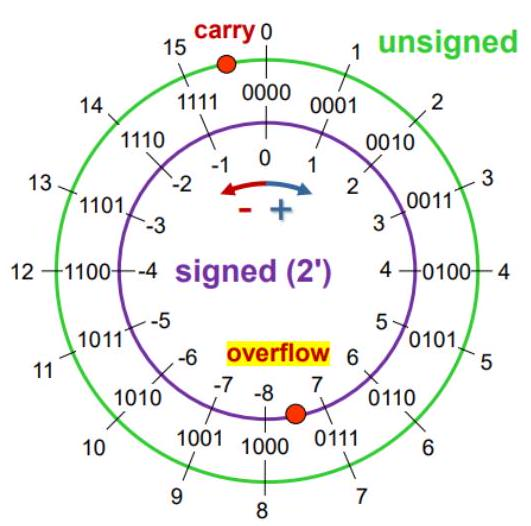
\includegraphics[width=\linewidth]{images/2024_12_29_79e6b22f503fb7b4f718g-04(2)}
\end{minipage}
\vspace{2mm}\\
\begin{minipage}[t]{0.4\linewidth}
Addition: C = 1 $\rightarrow$ Carry

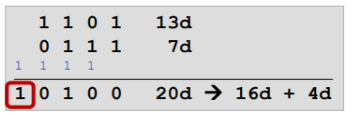
\includegraphics[width=\linewidth]{images/addcarry.png}
\end{minipage}
\begin{minipage}[t]{0.55\linewidth}
Subtraction: C = 0 $\rightarrow$ Borrow

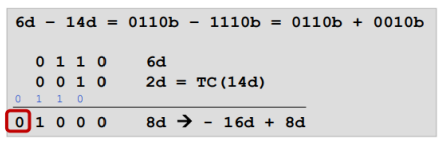
\includegraphics[width=\linewidth]{images/subborrow.png}
\end{minipage}
\end{concept}

\begin{example2}{Integer Ranges by Word Size}\\
\textbf{8-bit integers:}
\begin{itemize}
  \item Unsigned: 0 to 255 (0x00 to 0xFF)
  \item Signed: -128 to 127 (0x80 to 0x7F)
\end{itemize}

\textbf{16-bit integers:}
\begin{itemize}
  \item Unsigned: 0 to 65,535 (0x0000 to 0xFFFF)
  \item Signed: -32,768 to 32,767 (0x8000 to 0x7FFF)
\end{itemize}

\textbf{32-bit integers:}
\begin{itemize}
  \item Unsigned: 0 to 4,294,967,295 (0x00000000 to 0xFFFFFFFF)
  \item Signed: -2,147,483,648 to 2,147,483,647 (0x80000000 to 0x7FFFFFFF)
\end{itemize}
\end{example2}

\begin{KR}{Multi-Word Arithmetic}\\
Guidelines for operations on large numbers:

1. Addition sequence:
\begin{lstlisting}[language=armasm, style=basesmol]
    ; 64-bit addition (R1:R0 + R3:R2)
    ADDS    R0, R2          ; Add low words
    ADCS    R1, R3          ; Add high words with carry
\end{lstlisting}

2. Subtraction sequence:
\begin{lstlisting}[language=armasm, style=basesmol]
    ; 64-bit subtraction (R1:R0 - R3:R2)
    SUBS    R0, R2          ; Subtract low words
    SBCS    R1, R3          ; Subtract high words with borrow
\end{lstlisting}

3. Important considerations:
\begin{itemize}
  \item Start with least significant words
  \item Use carry-aware instructions for higher words
  \item Ensure proper register allocation
  \item Track flags through entire operation
\end{itemize}
\end{KR}

\begin{example2}{Multi-Word Addition}
Adding 96-bit values using ADCS:

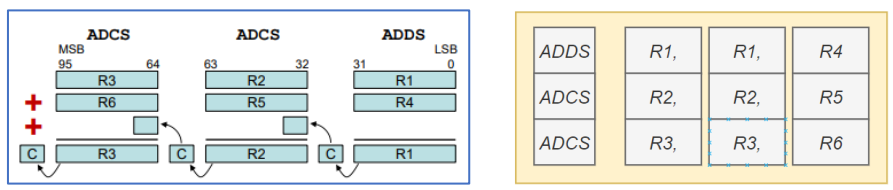
\includegraphics[width=\linewidth]{images/multiwordadd.png}

\begin{lstlisting}[language=armasm, style=basesmol]
ADDS R1, R1, R4    ; Add least significant words
ADCS R2, R2, R5    ; Add middle words with carry
ADCS R3, R3, R6    ; Add most significant words with carry
\end{lstlisting}
\end{example2}

\begin{example2}{Multi-Word Subtraction}
Subtracting 96-bit values using SBCS:

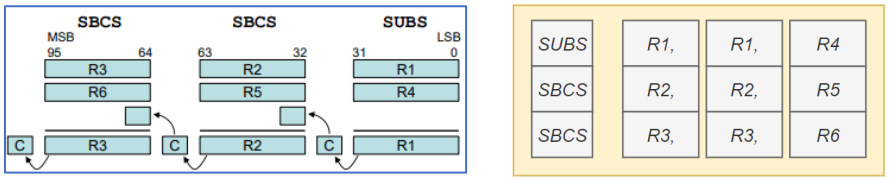
\includegraphics[width=\linewidth]{images/multiwordsub.png}

\begin{lstlisting}[language=armasm, style=basesmol]
SUBS R1, R1, R4    ; Subtract least significant words
SBCS R2, R2, R5    ; Subtract middle words with borrow
SBCS R3, R3, R6    ; Subtract most significant words with borrow
\end{lstlisting}
\end{example2}

\subsubsection{Flag Usage and Overflow Detection}

\begin{concept}{Processor Status Flags}\\
APSR (Application Program Status Register) contains important flags affected by arithmetic operations:
\begin{itemize}
  \item \textbf{N} (Negative): Set when result's MSB = 1, used for signed operations
  \item \textbf{Z} (Zero): Set when result = 0, used for both signed/unsigned
  \item \textbf{C} (Carry): Set when unsigned overflow occurs
  \item \textbf{V} (Overflow): Set when signed overflow occurs
\end{itemize}

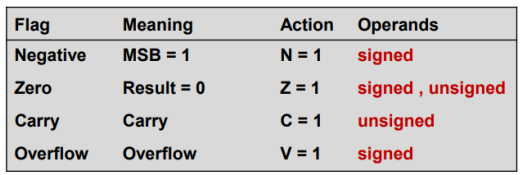
\includegraphics[width=\linewidth]{images/flags-arithmetic.png}

Instructions ending with 'S' modify these flags:
\begin{itemize}
  \item ADDS, SUBS, MOVS, LSLS
\end{itemize}
\end{concept}

\begin{KR}{Overflow Detection}\\
Steps to detect overflow in arithmetic operations:

1. For unsigned arithmetic (using C flag):
\begin{itemize}
  \item Addition: Check C flag (C=1 means overflow)
  \item Subtraction: Check C flag (C=0 means underflow)
\end{itemize}

2. For signed arithmetic (using V flag):
\begin{itemize}
  \item Addition: Check V flag for same-sign operands
  \item Subtraction: Check V flag for opposite-sign operands
\end{itemize}

Example:
\begin{lstlisting}[language=armasm, style=basesmol]
    ; Unsigned overflow detection
    ADDS    R0, R1          ; Perform addition
    BCS     overflow        ; Branch if carry set
    
    ; Signed overflow detection
    ADDS    R0, R1          ; Perform addition
    BVS     overflow        ; Branch if overflow set
\end{lstlisting}
\end{KR}

\begin{example2}{Flag Usage}
Examples of flag behavior:
\begin{lstlisting}[language=armasm, style=basesmol]
; Zero flag example
MOVS    R0, #5
SUBS    R0, #5          ; Z=1 (result is zero)

; Negative flag example
MOVS    R0, #1
SUBS    R0, #2          ; N=1 (result is negative)

; Carry flag example
MOVS    R0, #0xFF
ADDS    R0, #1          ; C=1 (unsigned overflow)

; Overflow flag example
MOVS    R0, #0x7F       ; Max positive 8-bit
ADDS    R0, #1          ; V=1 (signed overflow)
\end{lstlisting}
\end{example2}







